\documentclass{article}
\usepackage{arxiv}

\usepackage[utf8]{inputenc}
\usepackage[english, russian]{babel}
\usepackage[T1]{fontenc}
\usepackage{url}
\usepackage{booktabs}
\usepackage{amsfonts}
\usepackage{nicefrac}
\usepackage{microtype}
\usepackage{lipsum}
\usepackage{graphicx}
\usepackage{natbib}
\usepackage{doi}



\title{Автоматический подбор гиперпараметров моделей машинного обучения}

\author{ Надршена Вероника Рафиковна  \\
	МГУ им. М.В. Ломоносова\\
	ф-т ВМК, кафедра ММП\\
	% Pittsburgh, PA 15213 \\
	\texttt{s02190794@gse.cs.msu.ru} \\
	%% examples of more authors
	\And
	д.ф-м.н. Китов Виктор Владимирович\\
	МГУ им. М.В. Ломоносова\\
	ф-т ВМК, кафедра ММП\\
	% Santa Narimana, Levand \\
	%% \AND
	%% Coauthor \\
	%% Affiliation \\
	%% Address \\
	%% \texttt{email} \\
	%% \And
	%% Coauthor \\
	%% Affiliation \\
	%% Address \\
	%% \texttt{email} \\
	%% \And
	%% Coauthor \\
	%% Affiliation \\
	%% Address \\
	%% \texttt{email} \\
}
\date{}

\renewcommand{\shorttitle}{\textit{arXiv} Template}

%%% Add PDF metadata to help others organize their library
%%% Once the PDF is generated, you can check the metadata with
%%% $ pdfinfo template.pdf
\hypersetup{
pdftitle={Автоматический подбор гиперпараметров моделей машинного
обучения},
pdfsubject={q-bio.NC, q-bio.QM},
pdfauthor={David S.~Hippocampus, Elias D.~Striatum},
pdfkeywords={First keyword, Second keyword, More},
}

\begin{document}
\nocite{*}
\maketitle

\begin{abstract}
В рамках исследования проводилась оптимизация гиперпараметров классификатора метода опорных векторов (SVM) на наборе данных Wisconsin Diagnostic Breast Cancer (WDBC). Использовались различные техники оптимизации гиперпараметров, включая RandomizedSearchCV, направленный поиск в Optuna и BayesSearchCV из scikit-optimize, чтобы найти оптимальный набор параметров, максимизирующих точность модели.

\end{abstract}


\keywords{Grid Search \and Random Search \and байeсовская оптимизация}

\section{Введение}
В области машинного обучения процесс создания оптимальной модели часто включает в себя настройку гиперпараметров, что является критически важным этапом для достижения высокой производительности алгоритма. Гиперпараметры, в отличие от параметров модели, не обучаются непосредственно в процессе обучения, но они могут существенно влиять на качество итоговой модели. Например, коэффициент обучения, количество скрытых слоев в нейронной сети или параметры регуляризации — это лишь некоторые из гиперпараметров, которые нужно правильно выбрать.

Традиционные методы настройки гиперпараметров, такие как ручной подбор или сеточный поиск, могут быть трудоемкими и неэффективными, особенно при наличии большого числа гиперпараметров или при необходимости оптимизации сложных моделей \citep{bergstra2012}. В связи с этим автоматический подбор гиперпараметров становится все более популярным, так как он предлагает методы, способные автоматически и эффективно исследовать пространство гиперпараметров и находить оптимальные комбинации.

Алгоритмы автоматического подбора гиперпараметров, такие как байесовская оптимизация, генетические алгоритмы или градиентный подбор, показали свою эффективность в ряде исследований \citep{snoek2012, thornton2013}. Благодаря этому они стали неотъемлемой частью современных систем машинного обучения.

Однако, несмотря на прогресс в этой области, существует множество открытых вопросов и проблем. Основные трудности заключаются в масштабируемости алгоритмов, выборе подходящего метода для конкретной задачи или проблемах связанных со стабильностью и интерпретируемостью результатов.

Целью работы является изучение, анализ и сравнение современных методов автоматического подбора гиперпараметров, таких как Random Search, байесовская оптимизация и эволюционные алгоритмы, и определение их применимости и эффективности в различных задачах машинного обучения.

\section{Постановка задачи}
Рассмотрим множество моделей машинного обучения \( \mathcal{M} \). Для каждой модели \( m \in \mathcal{M} \) определим пространство гиперпараметров как \( \mathcal{H}_m \). Пусть \( L: \mathcal{M} \times \mathcal{H}_m \rightarrow \mathbb{R} \) представляет функцию потерь, которая оценивает качество соответствующей модели на заданном наборе данных при определенной комбинации гиперпараметров.

Задача автоматического подбора гиперпараметров может быть сформулирована следующим образом:

\[
(m^*, h^*) = \arg\min_{m \in \mathcal{M}, h_m \in \mathcal{H}_m} L(m, h_m).
\]

Цель состоит в том, чтобы найти такие \( m^* \) и \( h^* \), при которых функция потерь достигает минимального значения. Традиционные методы, такие как сеточный поиск, могут быть неэффективными в ситуациях с большим пространством гиперпараметров~\citep{bergstra2012}. С другой стороны, более современные методы, такие как байесовская оптимизация или эволюционные алгоритмы, предоставляют перспективные подходы к решению этой задачи~\citep{snoek2012, thornton2013}.



\section{Эксперимент}
Цель вычислительного эксперимента заключается в оптимизации гиперпараметров классификатора метода опорных векторов (SVM), применяемого к набору данных Wisconsin Diagnostic Breast Cancer (WDBC), полученного из OpenML. Набор данных состоит из диагностических измерений для случаев рака груди. Эксперимент включает использование различных техник оптимизации гиперпараметров, включая поиск по сетке с RandomizedSearchCV, направленный поиск Optuna и BayesSearchCV из scikit-optimize, для нахождения оптимального набора параметров, максимизирующих точность модели.

\subsection{Описание набора данных}
Набор данных, используемый в этом исследовании, - это широко используемый набор данных Wisconsin Diagnostic Breast Cancer (WDBC), полученный из репозитория OpenML. Этот набор данных включает диагностические измерения рака груди, каждый экземпляр представляет собой оцифрованное изображение мелкоигольной аспирационной биопсии (FNA) опухоли груди. Набор данных предоставляет характеристики, вычисленные на основе этих изображений, и использует их для классификации наблюдений как доброкачественные или злокачественные.

Набор данных содержит 569 экземпляров, каждый из которых имеет 30 числовых характеристик, описывающих свойства ядер клеток, присутствующих на изображениях. Эти характеристики организованы следующим образом:

\begin{itemize}
    \item Радиус (V1-V10): среднее расстояние от центра до точек на периметре.
    \item Текстура (V11-V20): стандартное отклонение значений градаций серого.
    \item Периметр (V21-V30): размер основной опухоли.
\end{itemize}

\begin{table}[h]
\centering
\caption{Пример набора данных WDBC}
\label{table:data}
\begin{tabular}{|c|c|c|c|c|c|c|c|c|c|c|}
\hline
Index & V1    & V2    & V3    & V4     & V5     & V6     & V7     & V8     & V9     & V10    \\ \hline
0     & 17.99 & 10.38 & 122.8 & 1001.0 & 0.1184 & 0.2776 & 0.3001 & 0.1471 & 0.2419 & 0.07871\\ \hline
1     & 20.57 & 17.77 & 132.9 & 1326.0 & 0.08474& 0.07864& 0.0869 & 0.07017& 0.1812 & 0.05667\\ \hline
2     & 19.69 & 21.25 & 130.0 & 1203.0 & 0.1096 & 0.1599 & 0.1974 & 0.1279 & 0.2069 & 0.05999\\ \hline
3     & 11.42 & 20.38 & 77.58 & 386.1  & 0.1425 & 0.2839 & 0.2414 & 0.1052 & 0.2597 & 0.09744\\ \hline
4     & 20.29 & 14.34 & 135.1 & 1297.0 & 0.1003 & 0.1328 & 0.198  & 0.1043 & 0.1809 & 0.05883\\ \hline
\end{tabular}
\end{table}

Эти характеристики охватывают такие аспекты, как текстура, периметр, площадь, гладкость, плотность, вогнутость и симметрия ядер клеток, среди прочих.

\begin{center}
    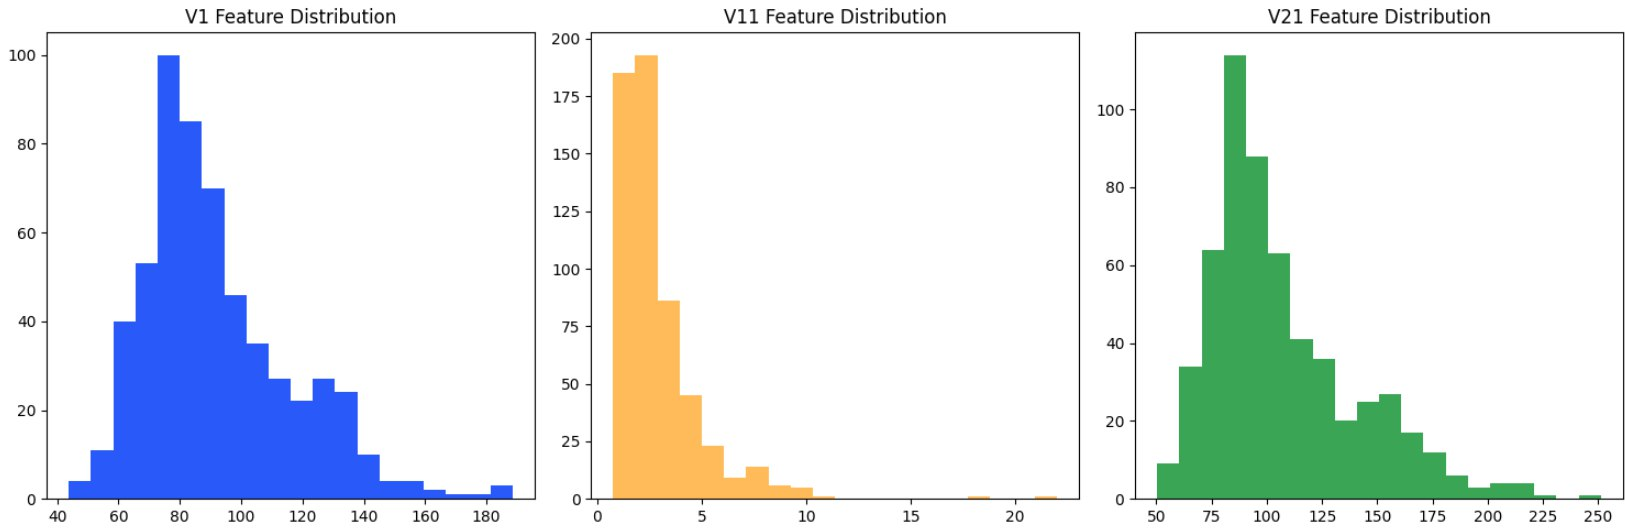
\includegraphics[width=\textwidth]{figures/parameters.jpg}
    \captionof{Примеры характеристик ядер клеток}
\end{center}

Для обеспечения воспроизводимости и целостности вычислительных экспериментов, набор данных случайным образом перемешивается с постоянным сидом. Затем он разделяется на обучающую выборку и тестовую выборку, при этом 40\% данных резервируются для тестирования с целью оценки производительности модели машинного обучения.

Эксперимент спроектирован так, чтобы быть надежным и повторяемым, с использованием стратифицированной выборки для поддержания распределения целей бинарной классификации между обучающей и тестовой выборками. Такой подход гарантирует, что обе подвыборки будут представлять общий набор данных, что позволяет более надежно оценивать способность модели к обобщению.



\subsection{Методология}
Методология эксперимента сосредоточена на применении и оптимизации классификатора метода опорных векторов (SVM) для набора данных WDBC. Алгоритм SVM выбран за его эффективность в задачах бинарной классификации и способность обрабатывать данные высокой размерности.

Оптимизация гиперпараметров SVM проводится с использованием трех различных стратегий:

\begin{enumerate}
\item \textbf{Случайный Поиск:} Выполняется случайный поиск по сетке с использованием RandomizedSearchCV из scikit-learn, исследуя заранее определенное пространство гиперпараметров. Эта стратегия поиска выбирает образцы из заданных распределений для гиперпараметров, таких как параметр регуляризации и тип ядра, обеспечивая базовый показатель производительности для настройки гиперпараметров.

\item \textbf{Оптимизация Optuna:} Используется продвинутая рамка оптимизации гиперпараметров Optuna для проведения более интенсивного поиска. Для интеллектуального навигации по пространству гиперпараметров на основе производительности предыдущих испытаний используется семплер Tree-structured Parzen Estimator (TPE) от Optuna, стремясь найти оптимальную конфигурацию за меньшее количество итераций.

\item \textbf{Байесовская Оптимизация:} Реализован BayesSearchCV из scikit-optimize для использования техник байесовской оптимизации. Этот подход моделирует пространство гиперпараметров с помощью гауссовского процесса и выбирает следующие гиперпараметры для оценки, балансируя между исследованием и использованием, стремясь минимизировать количество необходимых оценок.
\end{enumerate}



\subsection{Результаты}
\begin{center}
    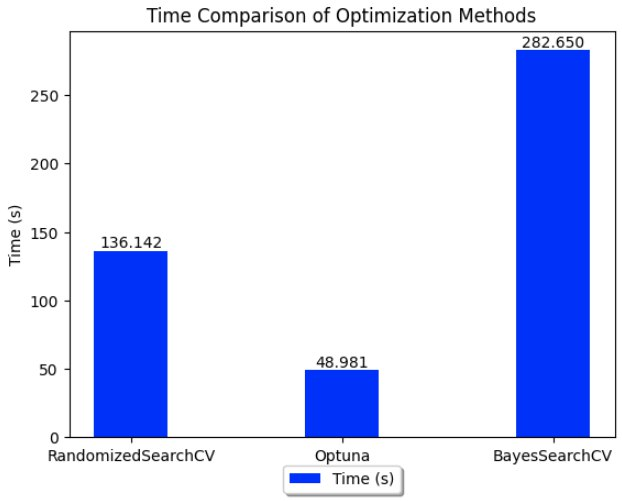
\includegraphics[width=\textwidth]{figures/time.jpg}
    \captionof{Время}
\end{center}

\begin{center}
    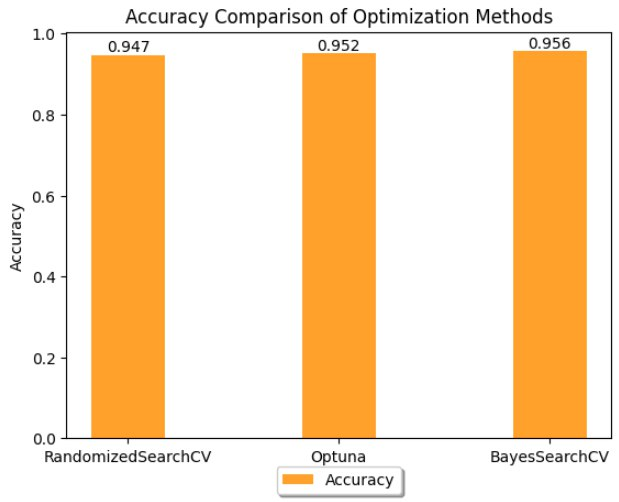
\includegraphics[width=\textwidth]{figures/accuracy.jpg}
    \captionof{Точность}
\end{center}

На этих графиках представлено сравнение трех различных методов оптимизации гиперпараметров, используемых для решения задачи машинного обучения: \texttt{RandomizedSearchCV}, \texttt{Optuna} и \texttt{BayesSearchCV}. На основе анализа представленных данных можно сделать несколько выводов:

\subsubsection{Времязатратность:}
\begin{itemize}
  \item \texttt{Optuna} --- самый быстрый метод, на поиск оптимальных параметров уходит всего 48,981 секунды.
  \item \texttt{RandomizedSearchCV} требует примерно в три раза больше времени, чем \texttt{Optuna}, и составляет 136,142 секунды.
  \item \texttt{BayesSearchCV} --- самый медленный, его время составляет 282,650 секунды, что почти в шесть раз больше, чем у \texttt{Optuna}, и примерно в два раза больше, чем у \texttt{RandomizedSearchCV}.
\end{itemize}

\subsubsection{Точность:}
\begin{itemize}
  \item Наибольшая точность у \texttt{BayesSearchCV} --- 0,956.
  \item Точность \texttt{Optuna} несколько ниже --- 0,952.
  \item \texttt{RandomizedSearchCV} имеет наименьшую точность среди всех трех методов --- 0,947.
\end{itemize}

\subsubsection{Наилучшие найденные параметры:}
Параметры, найденные каждым методом, отличаются, что свидетельствует о различных стратегиях поиска и достижении локального оптимума:
\begin{itemize}
  \item \texttt{RandomizedSearchCV} обнаружил высокое значение 'C' около 45,36, что говорит о меньшей силе регуляризации, а параметр 'kernel' установлен в значение 'linear'. В нем не используется параметр 'degree', так как он не имеет значения для линейного ядра, и задается значение 'gamma', которое также не используется линейными ядрами.
  \item \texttt{Optuna} также выбрала "линейное" ядро, но с гораздо меньшим значением 'C', равным примерно 1,299, что говорит о другом предпочтении регуляризации.
  \item \texttt{BayesSearchCV} выбрал "полиномиальное" ядро с чрезвычайно малым значением 'C' около 7,11e-08, "степенью" 2 для полиномиального ядра и "гаммой" около 1,566. Использование показателя "степень" здесь уместно, поскольку он характерен именно для ядра "poly".
\end{itemize}

\subsubsection{Выводы:}
Существует четкий компромисс между скоростью и точностью. Если \texttt{Optuna} является самой быстрой, то \texttt{BayesSearchCV}, несмотря на то, что она самая медленная, достигает самой высокой точности. Все методы выбрали различные гиперпараметры, что свидетельствует о том, что они по-разному исследуют пространство параметров. Различия в результатах также отражают лежащие в основе этих методов стратегии оптимизации. При выборе метода оптимизации необходимо учитывать специфические потребности своего приложения.

\bibliographystyle{unsrtnat}
\bibliography{references}

\end{document}
